\section{eo\-Eval\-Func$<$ EOT $>$ Class Template Reference}
\label{classeo_eval_func}\index{eoEvalFunc@{eoEvalFunc}}
Evaluate: takes one {\bf EO}{\rm (p.\,\pageref{class_e_o})} and sets its \char`\"{}fitness\char`\"{} property returning this fitness also.  


{\tt \#include $<$eo\-Eval\-Func.h$>$}

Inheritance diagram for eo\-Eval\-Func$<$ EOT $>$::\begin{figure}[H]
\begin{center}
\leavevmode
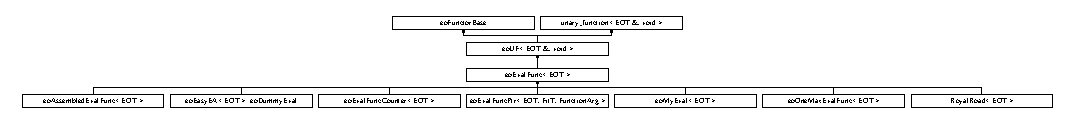
\includegraphics[height=1.22137cm]{classeo_eval_func}
\end{center}
\end{figure}
\subsection*{Public Types}
\begin{CompactItemize}
\item 
typedef {\bf EOT} {\bf EOType}\label{classeo_eval_func_w0}

\item 
typedef EOT::Fitness {\bf EOFit\-T}\label{classeo_eval_func_w1}

\end{CompactItemize}


\subsection{Detailed Description}
\subsubsection*{template$<$class EOT$>$ class eo\-Eval\-Func$<$ EOT $>$}

Evaluate: takes one {\bf EO}{\rm (p.\,\pageref{class_e_o})} and sets its \char`\"{}fitness\char`\"{} property returning this fitness also. 

That is why EOT is passed by non-const reference: it must be altered within evaluate.$\backslash$

The requirements on the types with which this class is to be instantiated with are null, or else, they depend on the particular class it's going to be applied to; {\bf EO}{\rm (p.\,\pageref{class_e_o})} does not impose any requirement on it. If you subclass this abstract class, and use it to evaluate an {\bf EO}{\rm (p.\,\pageref{class_e_o})}, the requirements on this {\bf EO}{\rm (p.\,\pageref{class_e_o})} will depend on the evaluator. 



Definition at line 41 of file eo\-Eval\-Func.h.

The documentation for this class was generated from the following file:\begin{CompactItemize}
\item 
eo\-Eval\-Func.h\end{CompactItemize}
